\begin{table}[h]
\caption{Specific rotations (\rotunits) of (\emph{S})-methyloxirane computed
in vacuum and shifts computed in solvents at the CCSD/aug-cc-pVDZ level
}
\begin{tabular*}{\linewidth}{@{\extracolsep{\fill}}cccccccc@{}}
  \hline \hline
&Vacuum &C$_6$H$_{12}$ &CCl$_4$&C$_6$H$_6$ &CH$_3$CH$_2$OH &CH$_3$CN  &H$_2$O \\
$\lambda$ (nm)
       &$[\alpha]_\omega$ &$\Delta [\alpha]_\omega$  &$\Delta [\alpha]_\omega$ 
&$\Delta [\alpha]_\omega$ &$\Delta [\alpha]_\omega$
&$\Delta [\alpha]_\omega$ &$\Delta [\alpha]_\omega$ \\
\hline
253 & 104.2 & -1.6  & -0.8 & -0.6 &+41.2 &+47.9 &+63.1 \\
302 & -42.8 &+11.5  &+13.3 &+13.6 &+52.0 &+56.5 &+66.2 \\
365 & -59.3 &+10.1  &+11.5 &+11.8 &+38.6 &+41.4 &+47.5 \\
436 & -50.1 & +7.5  & +8.5 & +8.7 &+27.2 &+29.0 &+33.0 \\
546 & -35.2 & +4.9  & +5.5 & +5.6 &+17.1 &+18.2 &+20.7 \\
578 & -31.9 & +4.3  & +4.9 & +5.0 &+15.2 &+16.2 &+18.4 \\
589 & -30.9 & +4.2  & +4.7 & +4.8 &+14.7 &+15.6 &+17.6 \\
\hline \hline
\end{tabular*}
\label{table:smo}
\end{table}

The case of methyloxirane perhaps best exemplifies the large role solvent
effects can play in optical rotation. Since the work of Kumata
\emph{et al.},\cite{Kumata:70} it has been recognized that the solvent
environment has a significant effect on the ORD curve of methyloxirane. 
These and subsequent experiments have revealed qualitatively different
shapes for the ORD curves in benzene compared to those in polar
solvents water and acetonitrile.\cite{Kumata:70,Wilson:05}
At a wavelength of 302 nm, the specific rotation of
(\emph{S})-methyloxirane in benzene is nearly -100 \rotunits, while, in water,
the measured rotation is around +60 \rotunits.\cite{Wilson:05} Specific rotations
measured at several wavelengths  on the ORD curve
for a variety of other solvents produce a range of
rotation values intermediate between these two solvents,
\cite{Kumata:70,Wilson:05} and available gas-phase measurements
lie closer to those in more polar solvents in this case.\cite{Wilson:05}

A variety of computational efforts have addressed the problem of
methyloxirane's specific rotation in solvent. Mennucci \emph{et al.}
\cite{Mennucci:02}
examined solvent effects on the rotation of several molecules,
including methyloxirane, presenting the first demonstration of
electronic structure calculations of optical rotation to employ 
PCM to model the solvent environment. Despite the success of PCM
in modeling a variety of molecular properties,\cite{Tomasi:05}
B3LYP\cite{Becke:93,Lee:88,Stephens:94} PCM calculations were incapable of reproducing the experimental
ordering of specific rotations in different solvents. B3LYP PCM
calculations have also been combined with zero-point vibrational
corrections in methyloxirane,\cite{Kongsted:08} resulting in
improvements in the computed solvent shifts in cyclohexane relative
to experiment. For more polar solvents, however, that methodology was
unable to model the correct relative shifts observed experimentally.
Beyond density functional theory, optical rotation of methyloxirane
in solution has also been investigated at the coupled-cluster level,
including correlation up to an approximation of triple excitations
in the CC3 method.\cite{Kongsted:05} In conjunction with a spherical
cavity dielectric model in CC/DC computations,\cite{Kongsted:05} 
those highly correlated methods also failed to predict the observed trends
across a variety of solvents.

Table \ref{table:smo} summarizes the results of CCSD/aug-cc-pVDZ specific
rotation values of (\emph{S})-methyloxirane computed in vacuum, as well
as in a variety of solvents treated as a continuum dielectric. The wavelengths
in the first column cover a range of values for which experimental measurements
are available. The CCSD/aug-cc-pVDZ specific rotation values for the isolated
molecule are given by the second column of Table \ref{table:smo}. At 253
nm, the vacuum rotation value is +104.2 \rotunits, becoming more negative
at -59.3 \rotunits \ as the wavelength increases to 365 nm. At longer wavelengths,
the vacuum rotation remains negative, reaching -30.9 \rotunits \ at 589 nm.
The remaining columns of Table \ref{table:smo} give the  solvent shifts computed
with the FGS model in combination with CCSD response calculations, relative
to the CCSD vacuum rotations. For the nonpolar solvents cyclohexane, carbon
tetrachloride, and benzene (third through fifth columns), the predicted
shifts are on the order of several \rotunits. The large positive rotation
at 253 nm is shifted only slightly smaller in each of these solvents, and none of
the shifts exceed 2 \rotunits. The negative specific rotations near 300 nm
all undergo larger shifts towards more positive values in the nonpolar environments, the magnitude of these shifts ranging from $+4$ to $+14$ \rotunits, with the
largest shifts due to the rotations calculated at 302 nm and 365 nm.
For the three polar solvents considered here (ethanol, acetonitrile, and water),
the specific rotation shifts relative to vacuum CCSD values are much larger.
At all wavelengths, the shifts are positive (last three columns of \ref{table:smo}). The predicted specific rotation shifts in water at
253 nm and 302 nm
exceed $+60$ \rotunits, a shift which is larger than the magnitude of any
of the negative vacuum specific rotation values above 300 nm.


\begin{figure}
\begin{subfigure}{.45\textwidth}
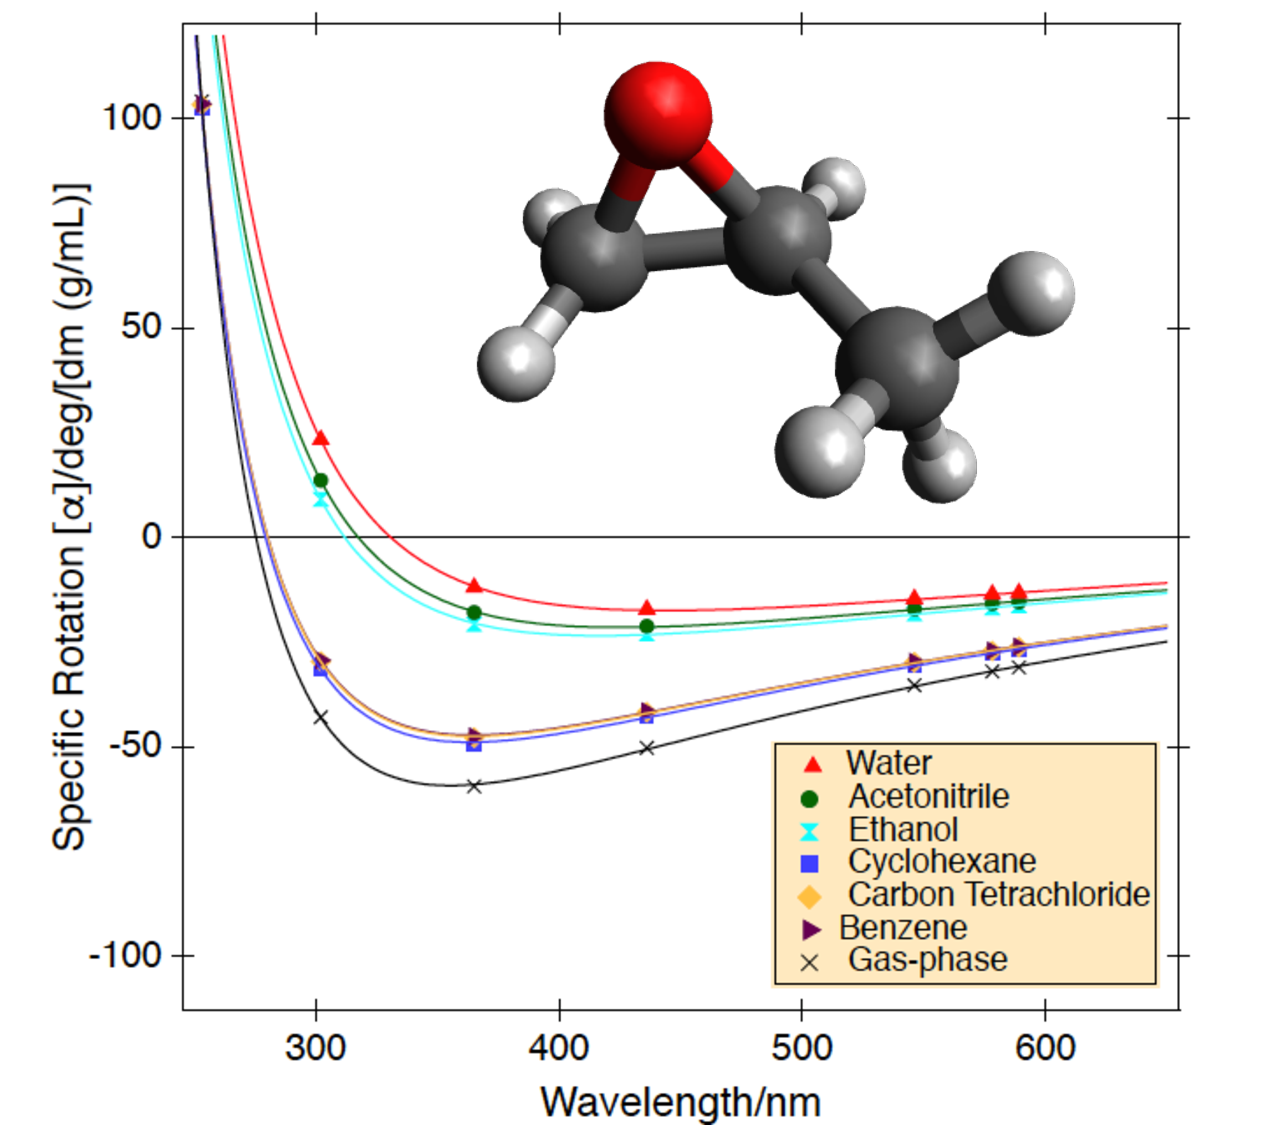
\includegraphics[width=2.5in]{figs/fig1a.pdf}
\caption*{\hspace{-1.25em}(a)}
\end{subfigure}
\hfill
\begin{subfigure}{.45\textwidth}
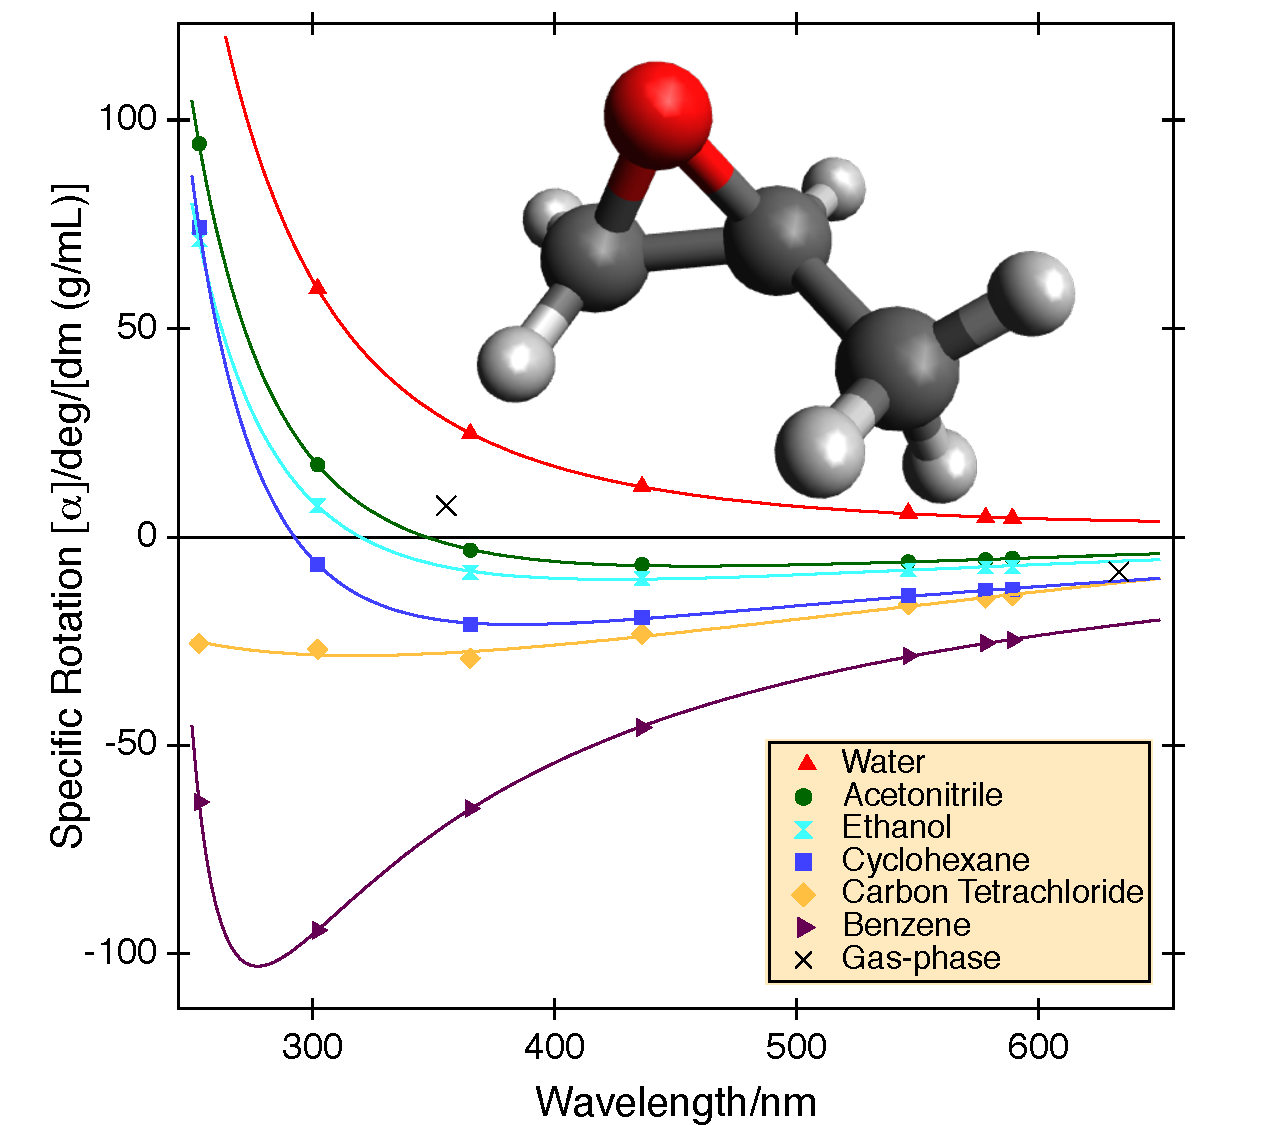
\includegraphics[width=2.5in]{figs/fig1b.pdf}
\caption*{\hspace{-1.25em}(b)}
\end{subfigure}
\caption{Optical rotatory dispersion curves of (\emph{S})-methyloxirane
(a) computed at the CCSD/aug-cc-pVDZ level with various solvents
and (b) from experimentally determined values\cite{Wilson:05}
}
\label{fig:smo}
\end{figure}

Figure \ref{fig:smo} displays the ORD curves for (\emph{S})-methyloxirane in
various solvents, including those computed at the CCSD/aug-cc-pVDZ level
in implicit solvent with the FGS model in Figure 1(a) and from experimental
determinations in Figure 1(b).
\cite{Wilson:05} The experimental rotation values display a wide
range
across all solvents, with the most polar solvents (water and acetonitrile)
showing positive rotations above 50 \rotunits\ at wavelengths
below 300 nm. In benzene,
the rotation of (\emph{S})-methyloxirane shifts to nearly -100 \rotunits\
in the same wavelength range experimentally. Comparing the CCSD/aug-cc-pVDZ
specific rotations computed in solution using the smooth FGS model (Figure
1(a)),
the relative ordering of the polar solvents water, acetonitrile, and ethanol
is correct, and the computed ORD curves display a qualitative agreement
with experiment for most of the polar solvents.
However, there are clearly major discrepancies in the calculated
and experimental curves. For example, the experimental ORD curve of (\emph{S})-methyloxirane
in water is positive at all wavelengths, while the values computed here
predict negative rotations above 302 nm. For the remaining solvents,
the sign of the rotation is correctly predicted, although the actual
values can deviate significantly from experiment, such as in benzene,
where the computed rotation value is too large at 302 nm by more than 60
\rotunits. In addition, because of the similar dielectric constants
of the nonpolar solvents here, the implicit solvent calculations are unable
to predict the variations seen experimentally among the ORD curves in nonpolar solvents.

In evaluating the quality of the CCSD calculations with the
FGS model, the shifts relative to vacuum are perhaps the most important,
since the absolute specific rotations in solution may benefit from
error cancellation in regards to basis set incompleteness, a lack of
vibrational corrections, etc. The experimental vacuum values\cite{Wilson:05}
are 7.49 \rotunits at 355 nm and -8.39 \rotunits at 633 nm (marked with
black X's in Figure 1). The CCSD/aug-cc-pVDZ vacuum values,
on the other hand, are represented by the most negative computed ORD curve.
At these two points, then, almost all of the computed shifts in Table 1
are in the wrong direction, with only the calculations in water solvent
correctly predicting positive shifts in the rotation. The unsatisfactory
performance of the CCSD shifts computed with the FGS model are in line
with previous efforts to apply continuum solvation to the problem of
methyloxirane's rotation in solution. The B3LYP PCM shifts
computed at 589 nm by Mennucci \emph{et al.}\cite{Mennucci:02}
agree with the CCSD FGS computed shifts for the nonpolar solvents
to within 2 \rotunits, while the acetonitrile shift computed in this work
are a bit more positive (by $+8$ \rotunits). Solvents shifts at 355
nm, also with B3LYP and PCM, were reported by Kongsted \emph{et al.}\cite{Kongsted:08}
and a similar shift was seen to that computed here at 365 nm in cyclohexane,
while the CCSD FGS results again predict larger shifts
in polar solvents compared to a DFT with PCM approach. 
Importantly, Kongsted \emph{et al.}
noted the importance of vibrational contributions to the shifts themselves,
as the effect was large enough in the case of cyclohexane to change the sign
of the computed shift at long wavelengths.\cite{Kongsted:08}
In contrast to the present CCSD results with the FGS model,
a previous attempt to model the solvents with a continuum model at the
CCSD level\cite{Kongsted:06} utilizing the CC/DC model predicts small, negative
shifts in the specific rotations of (\emph{S})-methyloxirane at 355 nm
for the nonpolar solvents examined here, in better accord with the experimental
picture and likely an improvement due to the CC/DC approach incorporating
the response of the solvent environment into the CC response equations.
\cite{Christiansen:99}

\begin{figure}
\begin{subfigure}{.4\textwidth}
\hspace{0.5in}
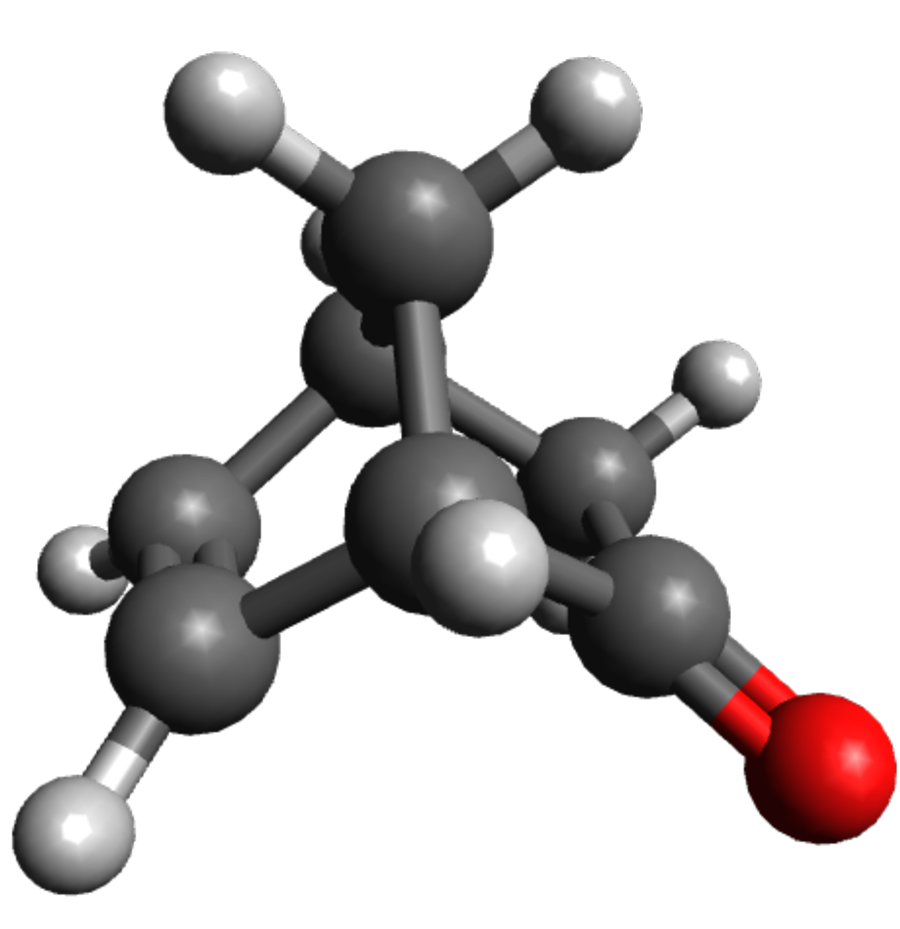
\includegraphics[width=1.75in]{figs/fig2a.pdf}
\caption*{\hspace{1.5em}(a)}
\end{subfigure}
\hfill
\begin{subfigure}{.4\textwidth}
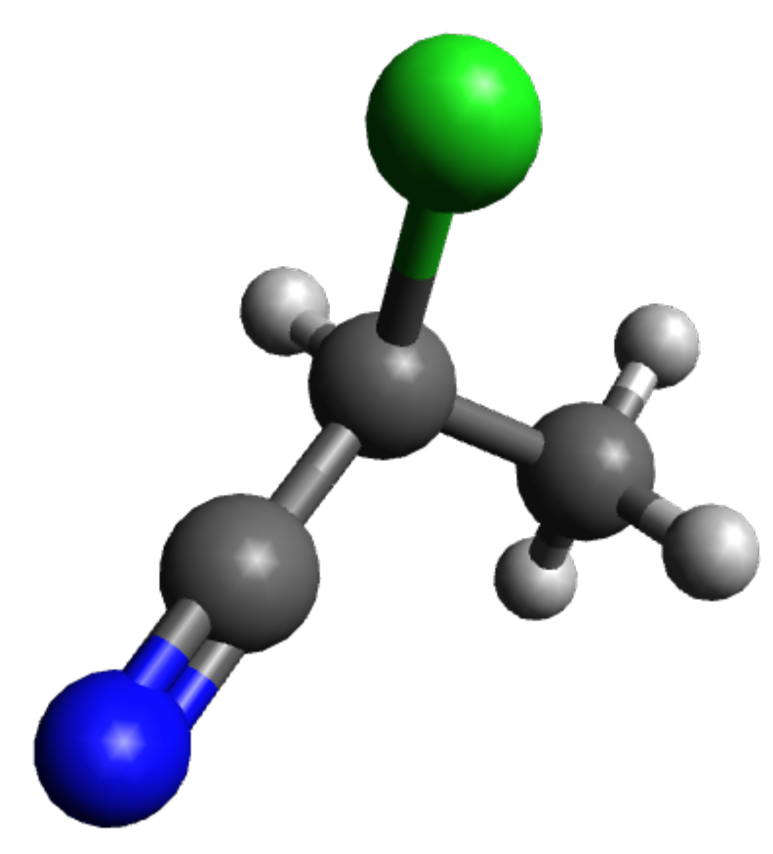
\includegraphics[width=1.75in]{figs/fig2b.pdf}
%\hfill
\caption*{\hspace{-5em}(b)}
\end{subfigure}
\caption{Two molecules studies in this work: (a) (\emph{1S},\emph{4S})-norbornenone
and (b) (\emph{S})-2-chloropropionitrile
}
\label{fig:other_molecules}
\end{figure}



Norbornenone is a molecule which has attracted theoretical interest due to
its very large-magnitude
specific rotation values relative to structurally similar chiral molecules.
\cite{Stephens:01,Ruud:03,Mach:11,Moore:12,Lahiri:13,Caricato:14}
The especially large rotation value has been analyzed in terms of the
excited state contributions\cite{Caricato:14}, as well as the contributions
from specific localized orbitals, and the lowest excited
state appears to be largely responsible for the sizable rotation,\cite{Caricato:14}
with a favorable alignment of the carbonyl and alkenyl groups playing a significant
role.\cite{Moore:12,Caricato:14} Modeling the
specific rotation of the isolated norbornenone molecule has been a challenge
and shows a strong dependence on theoretical method. DFT
\cite{Stephens:01,Ruud:03,Moore:12,Lahiri:13,Caricato:14}
and CC calculations\cite{Ruud:03,Mach:11,Lahiri:13} provide vastly
different rotation values, and at 355 nm, the experimental value of -6310
\rotunits \ is between B3LYP and CCSD results, which both deviate from
experiment by more than 2000 \rotunits.\cite{Lahiri:13}

\begin{table}[h]
\caption{Specific rotations (\rotunits) of (\emph{1S,4S})-norbornenone computed
in vacuum and shifts computed in solvents at the CCSD/aug-cc-pVDZ level
}
\begin{tabular*}{\linewidth}{@{\extracolsep{\fill}}cccccccc@{}}
  \hline \hline
& &\multicolumn{2}{c}{CCSD} &\multicolumn{2}{c}{PCM-B3LYP$^a$}
&\multicolumn{2}{c}{Experiment$^a$} \\
\cline{3-4} \cline{5-6} \cline{7-8}
&Vacuum &C$_6$H$_{12}$ &CH$_3$CN &C$_6$H$_{12}$ &CH$_3$CN 
&C$_6$H$_{12}$ &CH$_3$CN 
\\
$\lambda$ (nm) &$[\alpha]_\omega$
&$\Delta [\alpha]_\omega$ &$\Delta [\alpha]_\omega$ 
&$\Delta [\alpha]_\omega$ &$\Delta [\alpha]_\omega$ 
&$\Delta [\alpha]_\omega$ &$\Delta [\alpha]_\omega$ \\
\hline
355 &-3732.2 &+44.6 &+131.8 &-1066 &-855	&-2849  &-2297 \\
436 &-1429.4 &-4.9  &-15.0  &-- &--		&--  &-- \\
589 & -551.7 &-5.5  &-16.8  &-152 &-118		&-226  &-195 \\
633 & -454.5 &-4.8  &-14.9	&-125 &-96 	&-182  &-159 \\
\hline \hline
\multicolumn{8}{l}{$^a$ Reference \citenum{Lahiri:13}}
\end{tabular*}
\label{table:norb}
\end{table}

Norbornenone also undergoes a significant solvation effect, which is
under investigation here. Table \ref{table:norb} provides the calculated
CCSD/aug-cc-pVDZ vacuum rotations and shifts computed with the FGS
continuum treatment of solvent effects. For additional comparison, the
results of a B3LYP PCM treatment of implicit solvation have been included
as well.\cite{Lahiri:13} For the large negative rotation at 355 nm,
the CCSD FGS implementation predicts shifts in the positive
direction for both cyclohexane and acetonitrile solvents. Comparing
to the experimentally determined shifts in the last two columns of Table
\ref{table:norb}, these computed shifts are an order of magnitude smaller
than experiment, and the CCSD FGS results predict
a shift in the wrong direction. For the two rotation values that have been
measured in these solvents at 589 nm and 633 nm, the CCSD FGS calculations
predict
the correct direction of the shifts, but again the magnitudes are an order
of magnitude too small. The previously reported\cite{Lahiri:13} solvents shifts of 
norbornenone using B3LYP in conjunction with the PCM model perform
significantly better in regards to experiment. The PCM shifts predicted 
in cyclohexane and acetonitrile
are still underestimated with respect to the measured shifts, but
they are of the correct order of magnitude at each wavelength, and 
the cyclohexane shifts are correctly predicted to be larger in each case.


Because the calculated optical rotations in norbornenone are so 
dependent on the theoretical method, it is difficult to determine the
source of the poor performance of the implicit model used here without
continuum dielectric calculations performed at a level comparable to CCSD.
In order to further investigate shortcomings of the CCSD implementation of
the FGS model for optical rotation, we have performed specific rotation
calculations of (\emph{S})-2-chloropropionitrile, for which recent
experimental measurements and CCSD-PCM computed rotations have been
obtained by Aharon \emph{et al.}\cite{Aharon:18}
Table \ref{table:scpn} gives the vacuum CCSD/aug-cc-pVDZ specific rotation
values along with solvent shifts computed here with the FGS model,
the CCSD-PCM/aug-cc-pVDZ reported shifts, and those from experiment.\cite{Aharon:18}
For the vacuum values in the first column of data in Table \ref{table:scpn},
we note that the CCSD/aug-cc-pVDZ vacuum values for (\emph{S})-2-chloropropionitrile
are in very good agreement with the experimental values\cite{Aharon:18} 
of -37.9
\rotunits, -18.5 \rotunits, -8.1 \rotunits, and -6.8 \rotunits\ at the
wavelengths reported in the table. As with norbornenone, the CCSD method in conjunction with the FGS model significantly underestimates
the specific rotation shift at each wavelength. The CCSD-PCM computed shifts
reported in Table \ref{table:scpn} do not include the zero-point vibrational
corrections reported in Reference \citenum{Aharon:18} because we are interested
in the most straightforward comparison with the CCSD results computed
here to understand the drastically underestimated shifts. Even without
the zero-point vibrational corrections, which in most cases
improve the CCSD-PCM shifts relative to experiment, the solvent effects
on the optical rotation of (\emph{S})-2-chloropropionitrile appear to be
well described by CCSD-PCM, with the computed shifts always in the right
direction and typically within a few \rotunits\ of experimental values.
To understand the failure of the CCSD shifts computed with the FGS
model, we have performed additional PCM computations to investigate
whether the differences can be attributed to solute geometric effects,
differences in the implicit models' cavity definitions, or the 
solvent response treatment.

\begin{sidewaystable}[h]
\caption{Specific rotations (\rotunits) of (\emph{S})-2-chloropropionitrile
computed
in vacuum and shifts computed in solvents at the CCSD/aug-cc-pVDZ level
}
\footnotesize
\begin{tabular*}{\linewidth}{@{\extracolsep{\fill}}cccccc|cccc|cccc@{}}
  \hline \hline
& &\multicolumn{4}{c}{CCSD} &\multicolumn{4}{c}{CCSD-PCM$^{a,b}$}
&\multicolumn{4}{c}{Experiment$^a$} \\
\cline{2-6} \cline{7-10} \cline{11-14}
&Vacuum
&C$_6$H$_{12}$ &CH$_3$CN &C$_8$H$_{18}$O &CH$_3$OH 
&C$_6$H$_{12}$ &CH$_3$CN &C$_8$H$_{18}$O &CH$_3$OH 
&C$_6$H$_{12}$ &CH$_3$CN &C$_8$H$_{18}$O &CH$_3$OH  \\
$\lambda$(nm) &$[\alpha]_\omega$
&$\Delta [\alpha]_\omega$ &$\Delta [\alpha]_\omega$ 
&$\Delta [\alpha]_\omega$ &$\Delta [\alpha]_\omega$ 
&$\Delta [\alpha]_\omega$ &$\Delta [\alpha]_\omega$ 
&$\Delta [\alpha]_\omega$ &$\Delta [\alpha]_\omega$ 
&$\Delta [\alpha]_\omega$ &$\Delta [\alpha]_\omega$ 
&$\Delta [\alpha]_\omega$ &$\Delta [\alpha]_\omega$ \\
\hline
355 &-27.6  &-1.5  &-0.7 &-2.0 &-0.8 &-15.7 &-10.9 &-12.8 &-10.2  &-26.5 &-7.5 &-21.8 &-14.2 \\
437 &-15.4  &-0.9  &-0.7 &-1.4 &-0.7 &-9.4  &-6.6 &-7.6  &-6.2  &-17.8 &-6.4 &-15.1 &-10.4 \\
589 &-7.3  &-0.5  &-0.4 &-0.8 &-0.5 &-4.4  &-3.0 &-3.5  &-2.8  &-9.3  &-3.5 &-7.9  &-6.0 \\
633 &-6.2  &-0.4  &-0.4 &-0.7 &-0.4 &-3.9  &-2.7 &-3.1  &-2.5  &-7.8  &-3.1 &-6.9  &-5.1 \\
\hline \hline
\multicolumn{14}{l}{$^a$ Reference \citenum{Aharon:18}} \\
\multicolumn{14}{l}{$^b$ Zero-point vibrational corrections removed from
reported CCSD-PCM shift}
\end{tabular*}
\label{table:scpn}
\end{sidewaystable}




\begin{table}[h]
\caption{CCSD/aug-cc-pVDZ specific rotations solvents shifts
of (\emph{S})-2-chloropropionitrile computed with the FGS model and PCM
continuum models
}
\begin{tabular*}{\linewidth}{@{\extracolsep{\fill}}ccccc@{}}
  \hline \hline
  $\lambda$ (nm)
&$^\mathrm{vacuum}_\mathrm{geom}\Delta [\alpha]_\omega^\mathrm{FGS}$
&$^\mathrm{vacuum}_\mathrm{geom}\Delta [\alpha]_\omega^\mathrm{PCM-PTE}$
&$^\mathrm{solvent}_\mathrm{geom}\Delta [\alpha]_\omega^\mathrm{PCM-PTE}$ 
&$^\mathrm{solvent}_\mathrm{geom}\Delta [\alpha]_\omega^\mathrm{PCM,ab}$ \\
\hline
\multicolumn{5}{c}{Cyclohexane} \\
355 &-1.5 &-0.9 &-1.0 &-15.7 \\
437 &-0.9 &-0.6 &-0.6 &-9.4 \\
589 &-0.5 &-0.3 &-0.3 &-4.4 \\
633 &-0.4 &-0.3 &-0.3 &-3.9 \\
\hline
\multicolumn{5}{c}{Acetonitrile} \\
355 &-0.7 &-3.0 &-2.7 &-10.9 \\
437 &-0.7 &-2.0 &-1.6 &-6.6 \\
589 &-0.4 &-1.1 &-0.8 &-3.0 \\
633 &-0.4 &-0.9 &-0.7 &-2.7\\
\hline \hline
\multicolumn{5}{l}{$^a$Reference \citenum{Aharon:18}} \\
\multicolumn{5}{l}{$^b$ Zero-point vibrational corrections removed from
reported shift}
\end{tabular*}
\label{table:pcm}
\end{table}

In Table \ref{table:pcm}, the CCSD/aug-cc-pVDZ shifts computed using the
FGS model are compared to different computational protocol utilizing CCSD
in conjunction with PCM. For these PCM computations, the PTE approximation
is employed in the same manner as the FGS calculations. In other words, the
effect of the implicit solvent is only captured through the polarization of the
HF molecular orbitals, as well as the Fock matrix elements. In addition,
the CCSD-PCM-PTE specific rotation calculations were performed on 
(\emph{S})-2-chloropropionitrile geometries optimized in vacuum, as well as
in the corresponding solvent using PCM (2nd and 3rd columns of data in
Table \ref{table:pcm}). Comparing the first two columns of data in
Table \ref{table:pcm}, the CCSD-PCM-PTE cyclohexane shifts computed with the vacuum-
optimized geometry are seen to be very close
to those from the FGS model and, in fact, are slightly smaller than the
FGS shifts. The acetonitrile PCM-PTE shifts are of slightly
larger magnitude relative to FGS using the vacuum geometry. Examining
the CCSD-PCM-PTE shifts computed with PCM optimized geometries in the third
column of data in Table \ref{table:pcm}, the effect of geometry is seen to
have a minimal impact on the computed shifts. Capturing the solvent
effects at the Hartree-Fock level in the PTE approximation and, thus,
neglecting the solvent response to the electric and magnetic field
perturbations results in a significant underestimation of the solvent's role
in the specific rotation of (\emph{S})-2-chloropropionitrile, as evidenced by
the shifts computed with the fully coupled linear response CCSD-PCM-PTED
shifts from Reference \citenum{Aharon:18} (last column of Table \ref{table:pcm}),
which are an order of magnitude larger than each of the CCSD-PCM-PTE cyclohexane
shifts. This is reminiscent of the situation for frozen-density embedding
(FDE) potentials for modeling water solvent molecules in CC2 specific rotation calculations.\cite{Crawford:15}
As with the CCSD FGS calculations performed here, capturing the solvent
effects through FDE potentials incorporated into the Hartree-Fock reference state
proved inadequate for reproducing the results from explicit solvent calculations
due to the lack of solvent response. Unfortunately, a fully coupled implementation of
a coupled-cluster linear response (LR) scheme including implicit solvent results
in eight sets of coupled linear equations for perturbed CC $t$ and
$\lambda$ amplitudes and a significantly higher computational cost. Recently
introduced approximate schemes\cite{Caricato:18} for including solvent
response in the CC-LR
equations may offer a great advantage over PTE-type solvent treatments
at a reduced computational effort.\cite{Caricato:18}





